%%%%%%%%%%%%%%%%%%%%%%%%%%%%%%%%%%%%%%%%%
% a0poster Portrait Poster
% LaTeX Template
% Version 1.0 (22/06/13)
%
% The a0poster class was created by:
% Gerlinde Kettl and Matthias Weiser (tex@kettl.de)
% 
% This template has been downloaded from:
% http://www.LaTeXTemplates.com
%
% License:
% CC BY-NC-SA 3.0 (http://creativecommons.org/licenses/by-nc-sa/3.0/)
%
%%%%%%%%%%%%%%%%%%%%%%%%%%%%%%%%%%%%%%%%%

%----------------------------------------------------------------------------------------
%	PACKAGES AND OTHER DOCUMENT CONFIGURATIONS
%----------------------------------------------------------------------------------------

\documentclass[a0,portrait]{a0poster}

\usepackage{multicol} % This is so we can have multiple columns of text side-by-side
\columnsep=100pt % This is the amount of white space between the columns in the poster
\columnseprule=3pt % This is the thickness of the black line between the columns in the poster

\usepackage[svgnames]{xcolor} % Specify colors by their 'svgnames', for a full list of all colors available see here: http://www.latextemplates.com/svgnames-colors

\usepackage{times} % Use the times font
%\usepackage{palatino} % Uncomment to use the Palatino font

\usepackage{graphicx} % Required for including images
\graphicspath{{figures/}} % Location of the graphics files
\usepackage{booktabs} % Top and bottom rules for table
\usepackage[font=small,labelfont=bf]{caption} % Required for specifying captions to tables and figures
\usepackage{amsfonts, amsmath, amsthm, amssymb} % For math fonts, symbols and environments
\usepackage{wrapfig} % Allows wrapping text around tables and figures

\begin{document}

%----------------------------------------------------------------------------------------
%	POSTER HEADER 
%----------------------------------------------------------------------------------------

% The header is divided into two boxes:
% The first is 75% wide and houses the title, subtitle, names, university/organization and contact information
% The second is 25% wide and houses a logo for your university/organization or a photo of you
% The widths of these boxes can be easily edited to accommodate your content as you see fit

\begin{minipage}[b]{0.75\linewidth}
\veryHuge \color{NavyBlue} \textbf{Identificando Colines (\textit{Eleutherodactylus eileenae}) a partir de audios desordenados} \color{Black}\\ % Title
\Huge\textit{Sincronización y Procesamiento de Audios}\\[2cm] % Subtitle
\huge \textbf{Daniel Machado Pérez}\\[0.5cm] % Author(s)
\huge Tutores: Dr. Roberto Mulet, Dr. Milton Borroto\\[0.5cm] % Author(s)
\huge Facultad de Matemática y Computación, Universidad de La Habana\\[0.4cm] % University/organization
\Large \texttt{daniel.machado.0206@gmail.com}\\
\end{minipage}
%
\begin{minipage}[b]{0.25\linewidth}
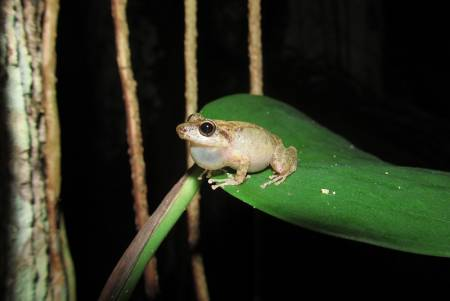
\includegraphics[width=20cm]{assets/elena.jpg}\\
\end{minipage}

\vspace{1cm} % A bit of extra whitespace between the header and poster content

%----------------------------------------------------------------------------------------

\begin{multicols}{3} % This is how many columns your poster will be broken into, a portrait poster is generally split into 2 columns

%----------------------------------------------------------------------------------------
%	ABSTRACT
%----------------------------------------------------------------------------------------

\color{Navy} % Navy color for the abstract

\renewcommand{\abstractname}{Resumen} % Uncomment to change the name of the abstract to something else
\begin{abstract}

    Este estudio analiza las secuencias de cantos de la 
    rana \textit{Eleutherodactylus eileenae}, 
    obtenidos mediante grabaciones de campo realizadas 
    con nueve micrófonos distribuidos alrededor de los 
    especímenes. Para identificar las secuencias 
    probables de los cantos se propone un método que 
    emplea mel-espectrogramas y análisis de las energías 
    temporales de las grabaciones. Para garantizar la sincronización de 
    los audios, se procedió con la obtención de
    los momentos de pico de energía y el cálculo de los 
    desfases con correlación cruzada utilizando un 
    archivo de referencia. Cada canto es conocido comúnmente como
    Colín (por comodidad, así llamaremos también a la especie), en imitación al sonido producido, en el que se emite
    una señal con frecuencia baja que denominaremos CO y una con frecuencia
    alta que llamaremos LIN. Los resultados 
    revelan patrones en la estructura del coro, donde 
    cada rana parece mantener una periodicidad consistente 
    entre cantos y ajustar las frecuencias en respuesta a 
    otros individuos.
\end{abstract}

%----------------------------------------------------------------------------------------
%	INTRODUCTION
%----------------------------------------------------------------------------------------

\color{SaddleBrown} % SaddleBrown color for the introduction

\section*{Introducción}

La rana \textit{Eleutherodactylus eileenae} (Dunn, 1926) es una especie endémica de Cuba \cite{Alonso:2001}. Su canto, que se caracteriza por emisiones de frecuencias bajas (CO) y altas (LIN), representa un objeto de estudio bioacústico único. Este trabajo propone un enfoque automatizado para identificar y analizar las secuencias de cantos de Colines a partir de grabaciones realizadas con nueve micrófonos distribuidos alrededor de los especímenes. Utilizando mel-espectrogramas, análisis de energías temporales y técnicas de correlación cruzada, se logra la sincronización de los audios y la separación de los cantos individuales. Este método no solo permite un análisis eficiente de los coros, sino que también abre nuevas posibilidades para estudiar su dinámica y estructura, abordando preguntas fundamentales sobre el comportamiento acústico y social de la especie.


%----------------------------------------------------------------------------------------
%	OBJECTIVES
%----------------------------------------------------------------------------------------

\color{DarkSlateGray} % DarkSlateGray color for the rest of the content

\section*{Objetivos}

\begin{enumerate}
\item Construir un dataset “limpio” donde sea más fácil obtener
estadísticas e interpretar los resultados.
\item Sincronizar los archivos de audio.
\item Distinguir los especímenes más cercanos a cada micrófono.
\item Identificar las secuencias probables de los cantos de Colines.
\item Analizar el comportamiento de las frecuencias en los coros.
\item Validar la consistencia del método propuesto.
\end{enumerate}

%----------------------------------------------------------------------------------------
%	MATERIALS AND METHODS
%----------------------------------------------------------------------------------------

\section*{Materiales y Métodos}

Se cuenta con el dataset de las grabaciones hechas
por los 9 micrófonos, cuya ubicación geográfica se representa en la Figura 1.

\begin{center}\vspace{0.1cm}
    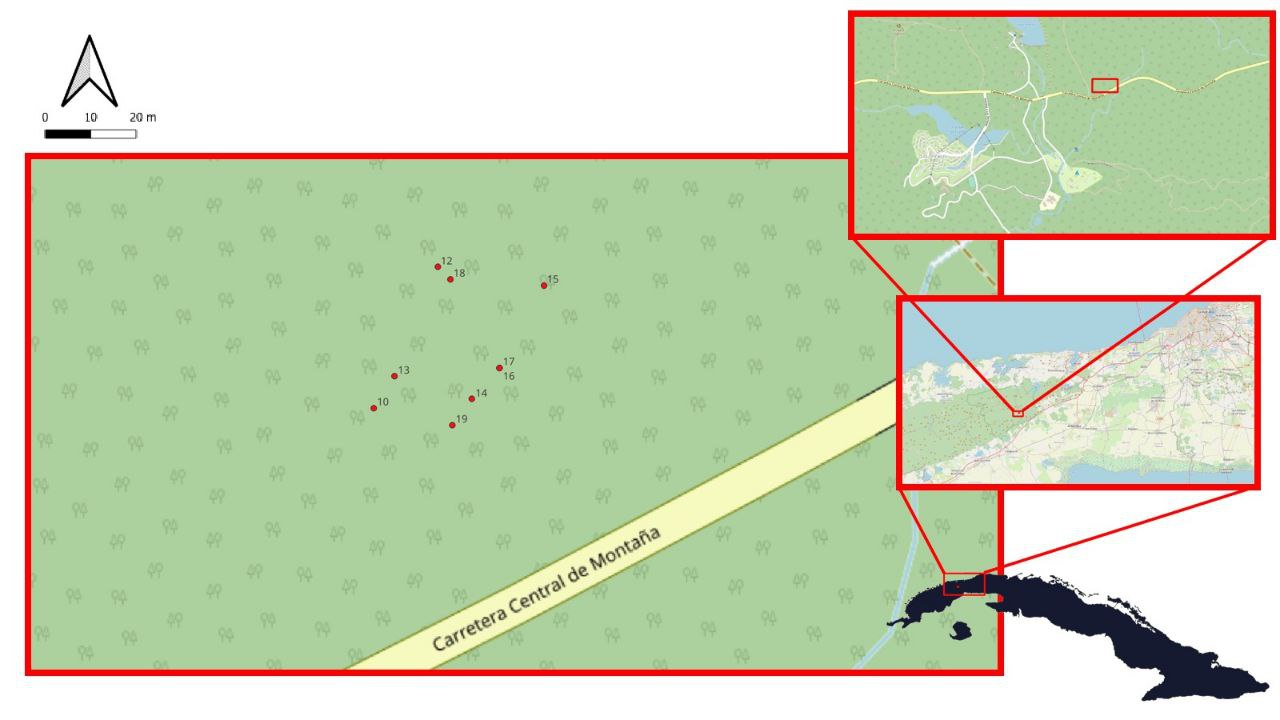
\includegraphics[width=0.8\linewidth]{assets/mic_map.jpg}
    \captionof{figure}{\color{Green} Distribución Geográfica de los Micrófonos.}
\end{center}\vspace{0.1cm}
 
Estas se realizaron durante 3 días,
a partir de las 18:00 hasta las 06:00 horas del día siguiente, donde de cada hora se registraron 58 minutos
y se descansaron 2. Los dispositivos se activaron remotamente y al mismo tiempo. Para lo que se presenta, se utilizó la información captada el día 21 de octubre de 2023 a las 19:00 horas.
Cada audio se representó y procesó a través de su mel-espectrograma. \cite{mel} Un ejemplo de ello se muestra en la Figura 2.


\begin{center}\vspace{0.1cm}
    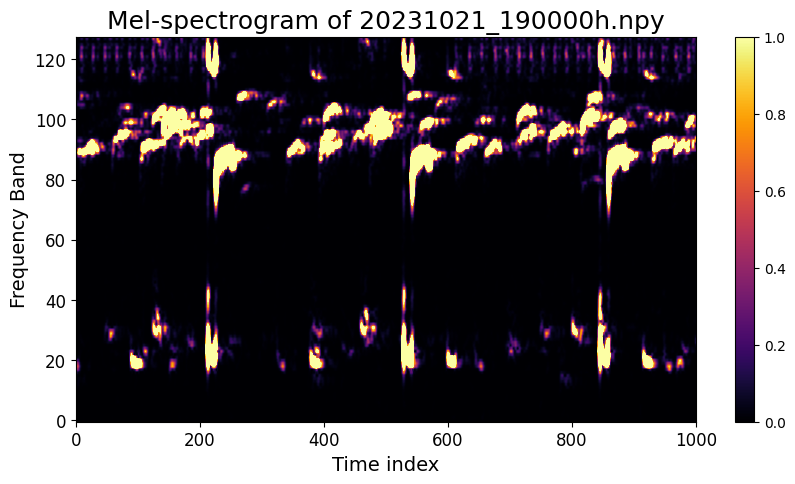
\includegraphics[width=0.8\linewidth]{assets/mel-spectrogram.png}
    \captionof{figure}{\color{Green} Mel-espectrograma del archivo \textit{h}}
\end{center}\vspace{0.1cm}

El proceso de sinconización comienza con la identificación de un archivo pivote,
que debe contener una señal que hayan captado todos los micrófonos y en un rango de bandas de frecuencias
lo más `limpio' posible. Luego se procede con el cálculo de las energías temporales con la siguiente fórmula, donde $E_j$ es el valor de la energía en el instante de tiempo $j$, $a_{ij}$ es la intensidad en el instante de tiempo $j$ y la banda de frecuencia $i$ en el mel-espectrograma correspondiente.:

\begin{equation*}
	E_j = \sum_{i=0} a_{ij}^{2}, \forall j     \cite{Jurafsky:2008}
\end{equation*} 

Luego se procede con la eliminación de ruido y la identificación de picos de energía. Sobre esa data se aplica \textbf{Correlación Cruzada}, entre cada archivo y el archivo pivote. El valor de \textit{lag} o desfase es el que maximiza la Correlación:

\begin{equation*}
	CC = \sum_{i=0}^{n} a_{i}b_{i},     \cite{Bourke:1996}
\end{equation*} 

Donde $a_i$ y $b_i$ son los valores en el índice $i$ de los \textit{arrays} sobre los que se aplica la Correlación. Finalmente el resutado es como el que se muestra en la Figura 3.

\begin{center}\vspace{0.1cm}
    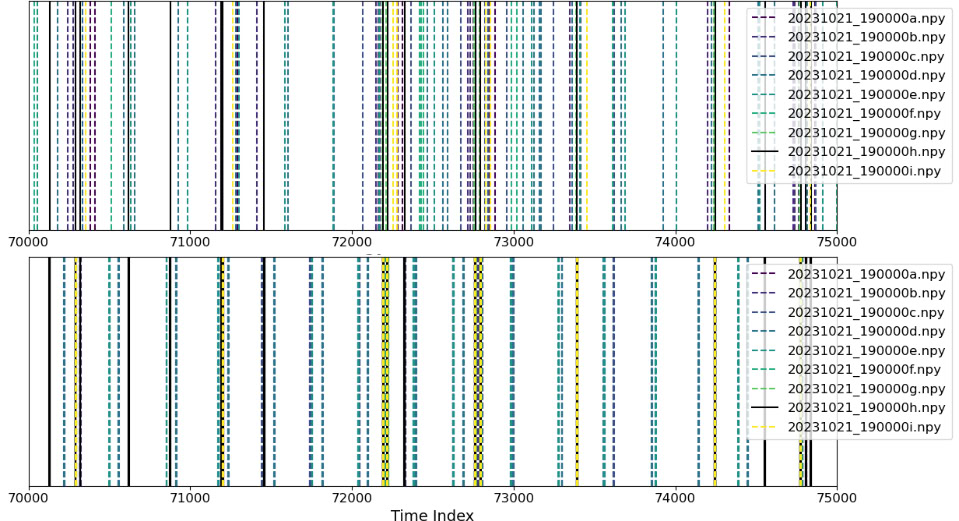
\includegraphics[width=0.8\linewidth]{assets/peaks_alignment.jpg}
    \captionof{figure}{\color{Green} Resultado de la Sincronización.}
\end{center}\vspace{0.1cm}

Luego se procede con la distinción del Colín más cercano a cada micrófono. Para ello se propone un método que se sustenta en las siguientes hipótesis:
\begin{itemize}
    \item Para cada micrófono, los cantos del individuo más cercano deben ser registrados con las mayores energías relativas a dicho micrófono.
    \item Si en cada uno se identifican las energías grandes y se elimina la información de esos cantos de las demás grabaciones, se obtendrán por separado los datos que se buscan.
\end{itemize}

\begin{center}\vspace{0.1cm}
    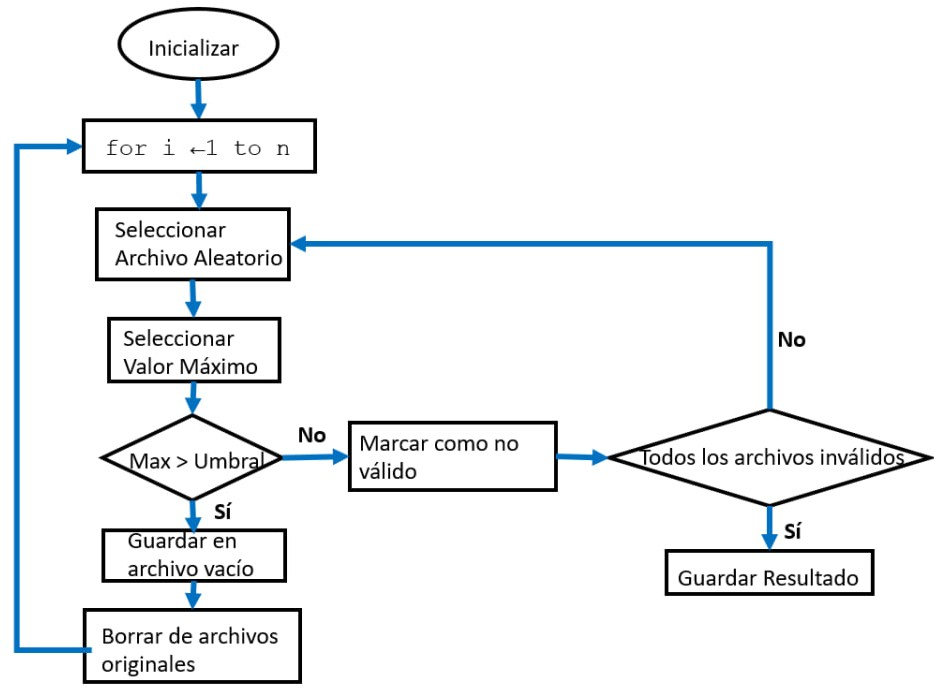
\includegraphics[width=0.8\linewidth]{assets/algorithm.jpg}
    \captionof{figure}{\color{Green} Esquema del método para distinción de cantos cercanos a micrófonos.}
\end{center}\vspace{0.1cm}
%------------------------------------------------


%----------------------------------------------------------------------------------------
%	RESULTS 
%----------------------------------------------------------------------------------------

\section*{Resultados}

Luego de tener la información de los cantos del Colín cercano a cada micrófono, podemos construir los coros, como se muestra en la Figura 5.
\begin{center}\vspace{0.1cm}
    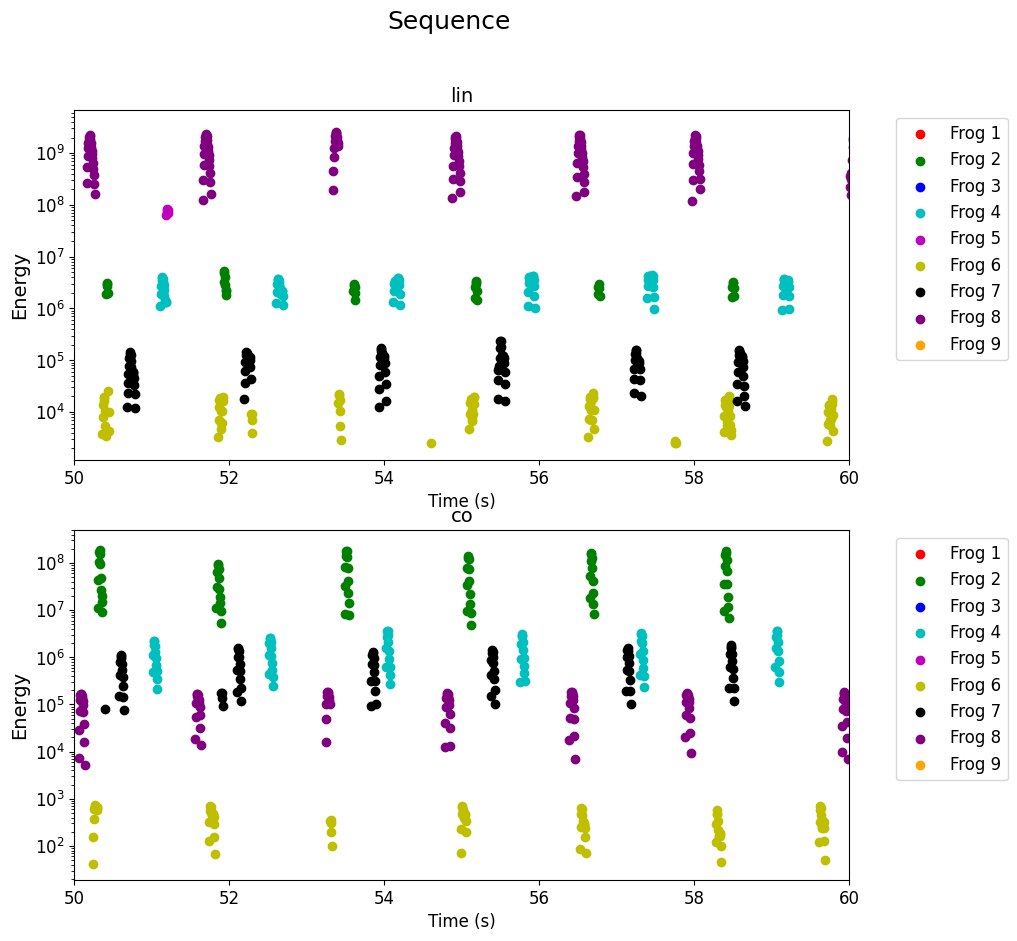
\includegraphics[width=0.8\linewidth]{assets/sequence.png}
    \captionof{figure}{\color{Green} Secuencia de cantos.}
\end{center}\vspace{0.1cm}

Además podemos conocer el comportamiento en cuanto a la frecuencia que manifiesta cada rana.
\begin{center}\vspace{1cm}
    \begin{minipage}{0.45\linewidth}
        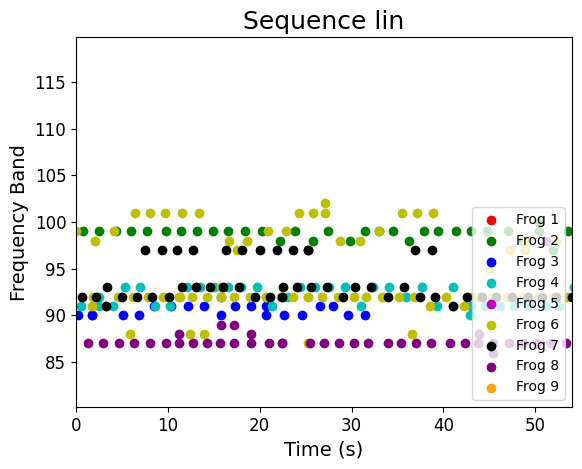
\includegraphics[width=\linewidth]{assets/frequencylin.png}
        \captionof{figure}{\color{Green} Frecuencia de los LIN.}
    \end{minipage}
    \hspace{0.05\linewidth}
    \begin{minipage}{0.45\linewidth}
        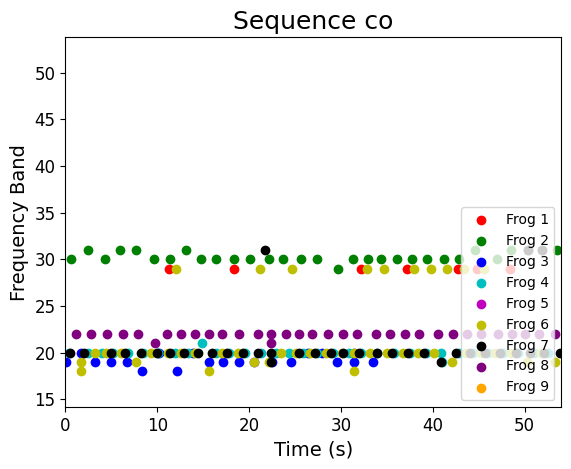
\includegraphics[width=\linewidth]{assets/frequencyco.png}
        \captionof{figure}{\color{Green} Frecuencia de los CO.}
    \end{minipage}
\end{center}\vspace{0.1cm}

De lo observado en las Figuras 6 y 7 se puede formular la hipótesis de que las ranas regulan la frecuencia de sus cantos en dependencia de las frecuencias de los demás miembros del coro, buscando baja superposición y tal vez mayor distinguibilidad.\\

Para validar la consistencia del algoritmo, se ejecutaron 10 \space corridas independientes y se hizo un análisis de correlación entre cada par de \textit{arrays} resultantes, también utilizando Correlación Cruzada. 
El resultado puede observarse en la Figura 8, donde en cada fila de la matriz se resaltan en rojo los 10 mayores valores de correlación, y los \textit{arrays} están organizados primero por audio y luego por corrida. 
Es decir, las 10 primeras filas corresponden al \textit{array} resultante del audio 1 en cada una de las 10 corridas, las siguientes 10 filas al \textit{array} del audio 2 en las 10 corridas y así consecutivamente.
De la misma forma están organizados en las columnas.
Como se observa, la mayor correlación se concentra entre los \textit{arrays} del mismo audio en las 10 corridas, probando que el algoritmo es consistente.  


\begin{center}\vspace{0.1cm}
    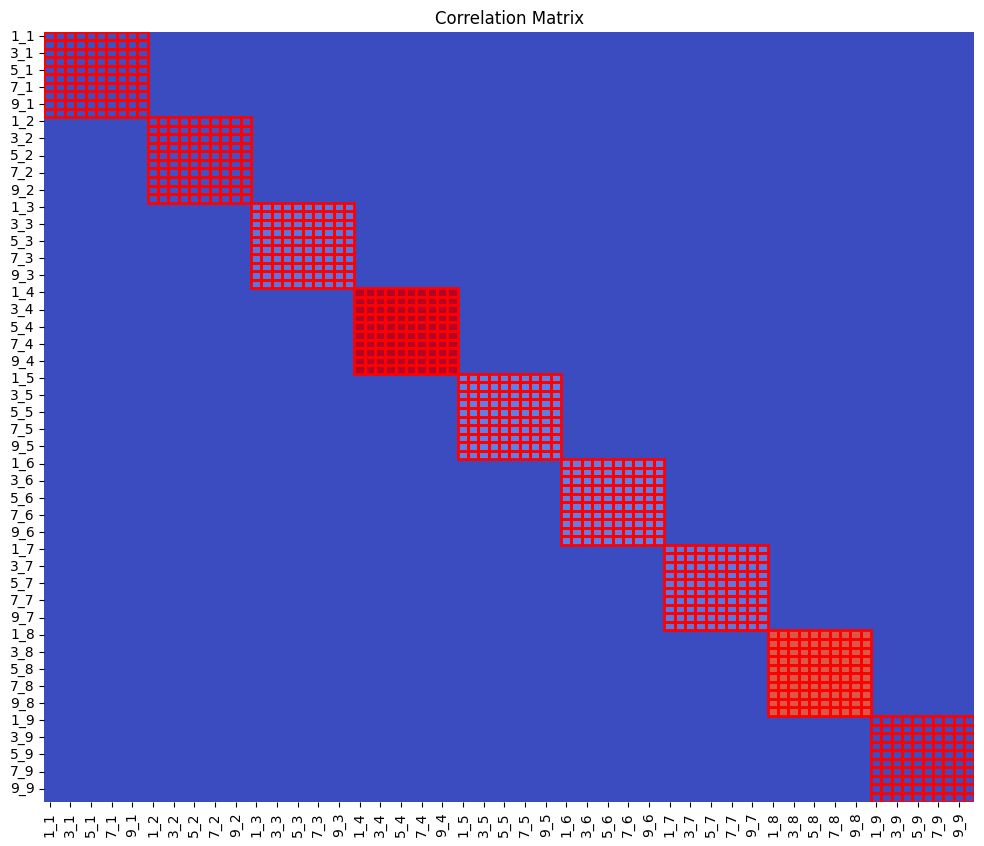
\includegraphics[width=0.7\linewidth]{assets/correlation_matrix.png}
    \captionof{figure}{\color{Green} Matriz de Correlación entre corridas distintas del Algoritmo}
\end{center}\vspace{0.1cm}

%----------------------------------------------------------------------------------------
%	CONCLUSIONS
%----------------------------------------------------------------------------------------

\color{SaddleBrown} % SaddleBrown color for the conclusions to make them stand out

\section*{Conclusiones}

\begin{itemize}
\item Se diseñó un método semi-automático de sincronización \space \space \space \space \space usando Correlación Cruzada, con resultados positivos.
\item Se diseñó un método automático para distinguir especímenes cercanos a micrófonos, del cual se logró validar su consistencia y efectividad.
\item Se construyó un dataset “limpio” que permitió obtener la secuencia de cantos y el comportamiento en frecuencia.
\end{itemize}

\color{DarkSlateGray} % Set the color back to DarkSlateGray for the rest of the content

%----------------------------------------------------------------------------------------
%	FORTHCOMING RESEARCH
%----------------------------------------------------------------------------------------

\section*{Líneas Futuras de Investigación}

\begin{itemize}
    \item Análisis de la hipótesis de que los Colines modifican su registro de frecuencia para diferenciarse de los demás cantos del coro.
    \item Análisis de causalidad, para estudiar la posibilidad de que en un coro existan individuos que manifiesten un papel protagónico en su estructura.
\end{itemize}
 %----------------------------------------------------------------------------------------
%	REFERENCES
%----------------------------------------------------------------------------------------

\renewcommand{\refname}{Referencias} % Change the title of the references section
\nocite{*} % Print all references regardless of whether they were cited in the poster or not
\bibliographystyle{plain} % Plain referencing style
\bibliography{build/sample.bib} % Use the example bibliography file sample.bib

%----------------------------------------------------------------------------------------
%	ACKNOWLEDGEMENTS
%----------------------------------------------------------------------------------------

\section*{Agradecimientos}

Al Dr. Roberto Alonso, por sus consejos sobre el comportamiento de la especie y por proveernos de los datos.
%----------------------------------------------------------------------------------------

\end{multicols}
\end{document}